The process that our experiment undertook was iterative. Obstacles in the analysis showed the need to develop tools that helped us to make the process less cumbersome. In the same way that in the previous chapter we explored the flow of ideas that led to our pipeline design, here we will explain how data shaped our experimental process.\\

The purpose of training a model, is to provide a faithful representation of the  studied phenomena, but how do we know that this description is correct? We need to validate the relationship between the outcome of the model and the data that we have at hand. Validation must be carefully crafted to obtain accurate results. In other words we need to control the variables that might affect the outcome of the experiment so we can isolate the phenomena that we are studying.\\

To have a complete picture of how our approach is compared with other classical techniques from  computer vision, we trained other models to test their performance against our novel approach. This exercise gave us some insight on the feasibility of a real world implementation.\\


\section{Exploratory analysis}

During the week following the Chiapas earthquake of September 7, 2017, several drones captured images from three different towns in the state of Oaxaca. We obtained those images from CENAPRED. The ensemble consisted of 1134 images from Juchit\'an de Zaragoza (Figure \ref{fig:juchitan}), 727 images from Santa Mar\'ia Xadani (Figure \ref{fig:santamaria}), and 1872 images from Uni\'on Hidalgo (Figure \ref{fig:union}).\\

\begin{figure}[!h]
  \centering
    \begin{subfigure}{.8\textwidth}
        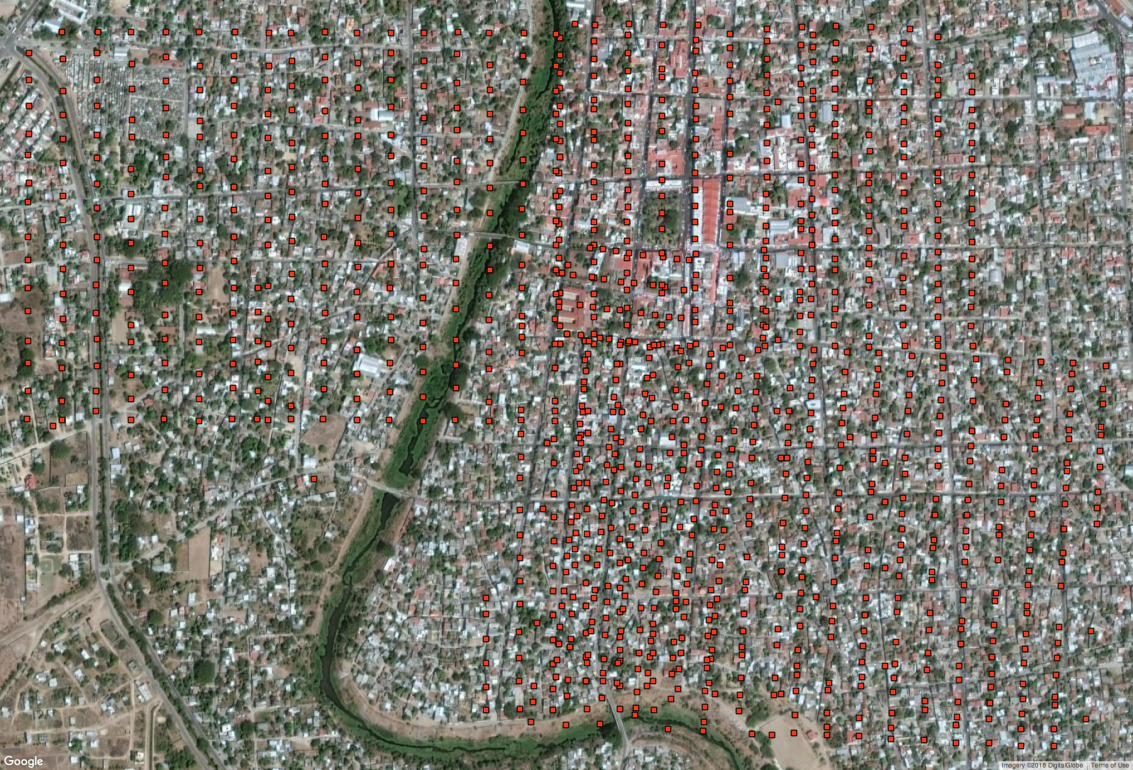
\includegraphics[width=\textwidth]{images/juchitan-satellite.jpg}
    \end{subfigure}
    \begin{subfigure}{.8\textwidth}
        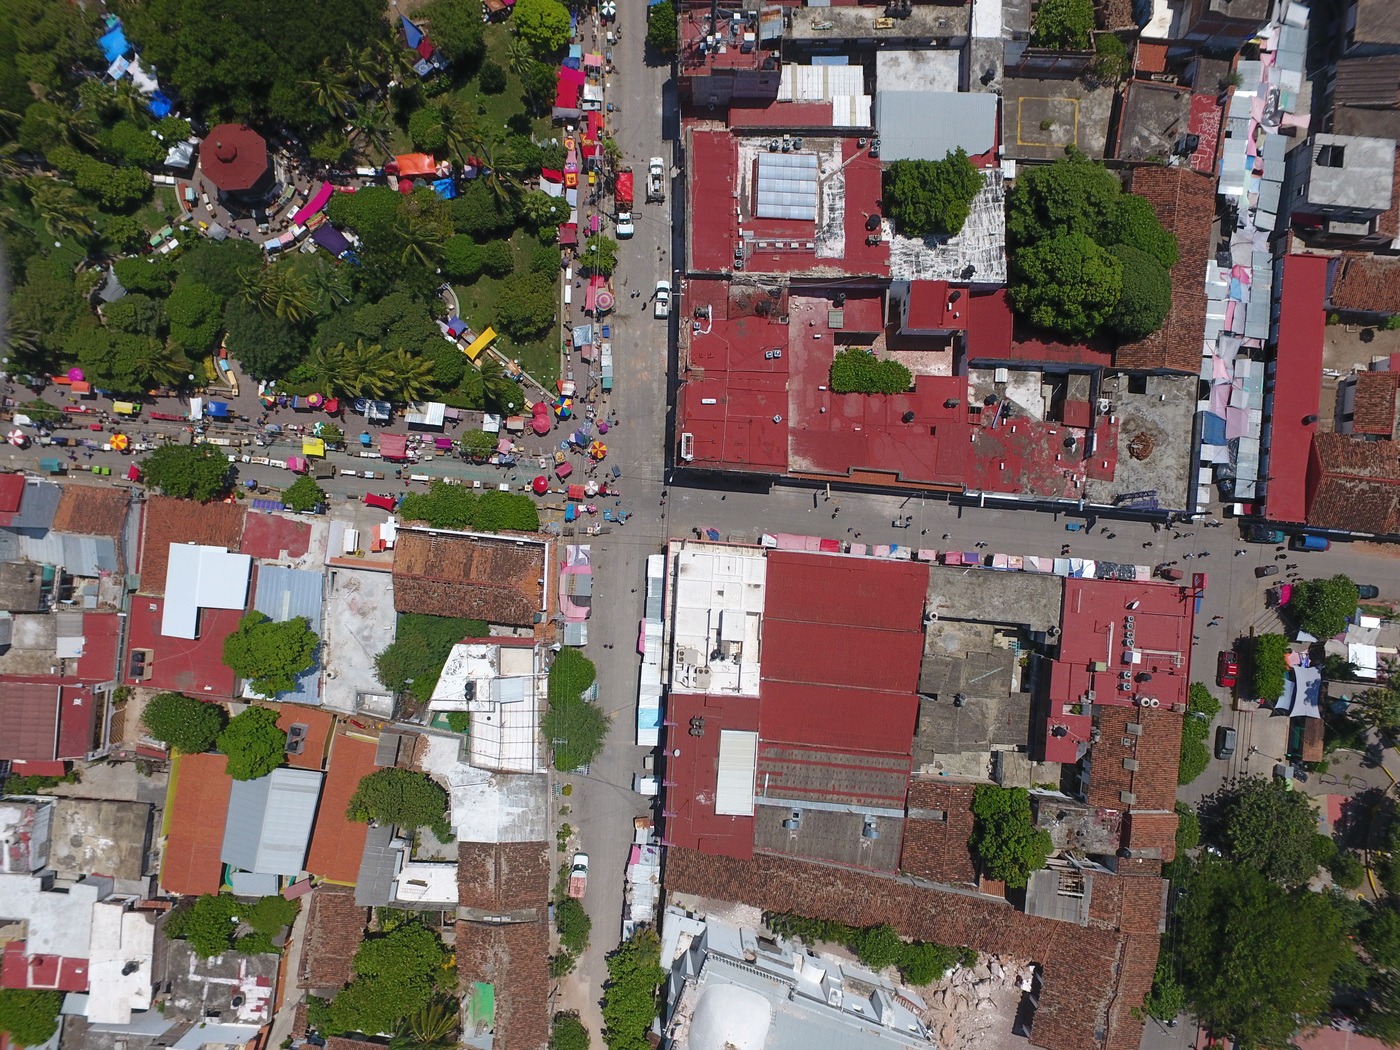
\includegraphics[width=\textwidth]{images/juchitan-sample.jpg}
    \end{subfigure}
  \caption{Juchit\'an de Zaragoza.}
  \label{fig:juchitan}
\end{figure}

\begin{figure}[!h]
  \centering
    \begin{subfigure}{.8\textwidth}
        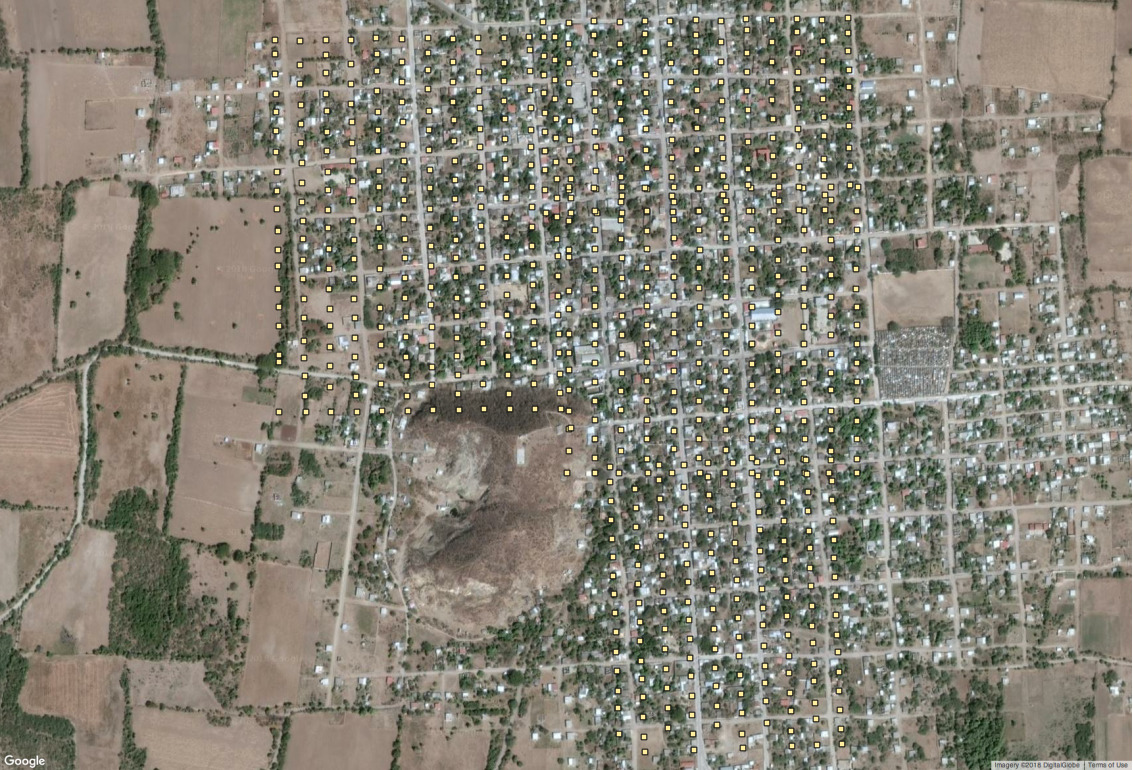
\includegraphics[width=\textwidth]{images/santamaria-satellite.jpg}
    \end{subfigure}
    \begin{subfigure}{.8\textwidth}
        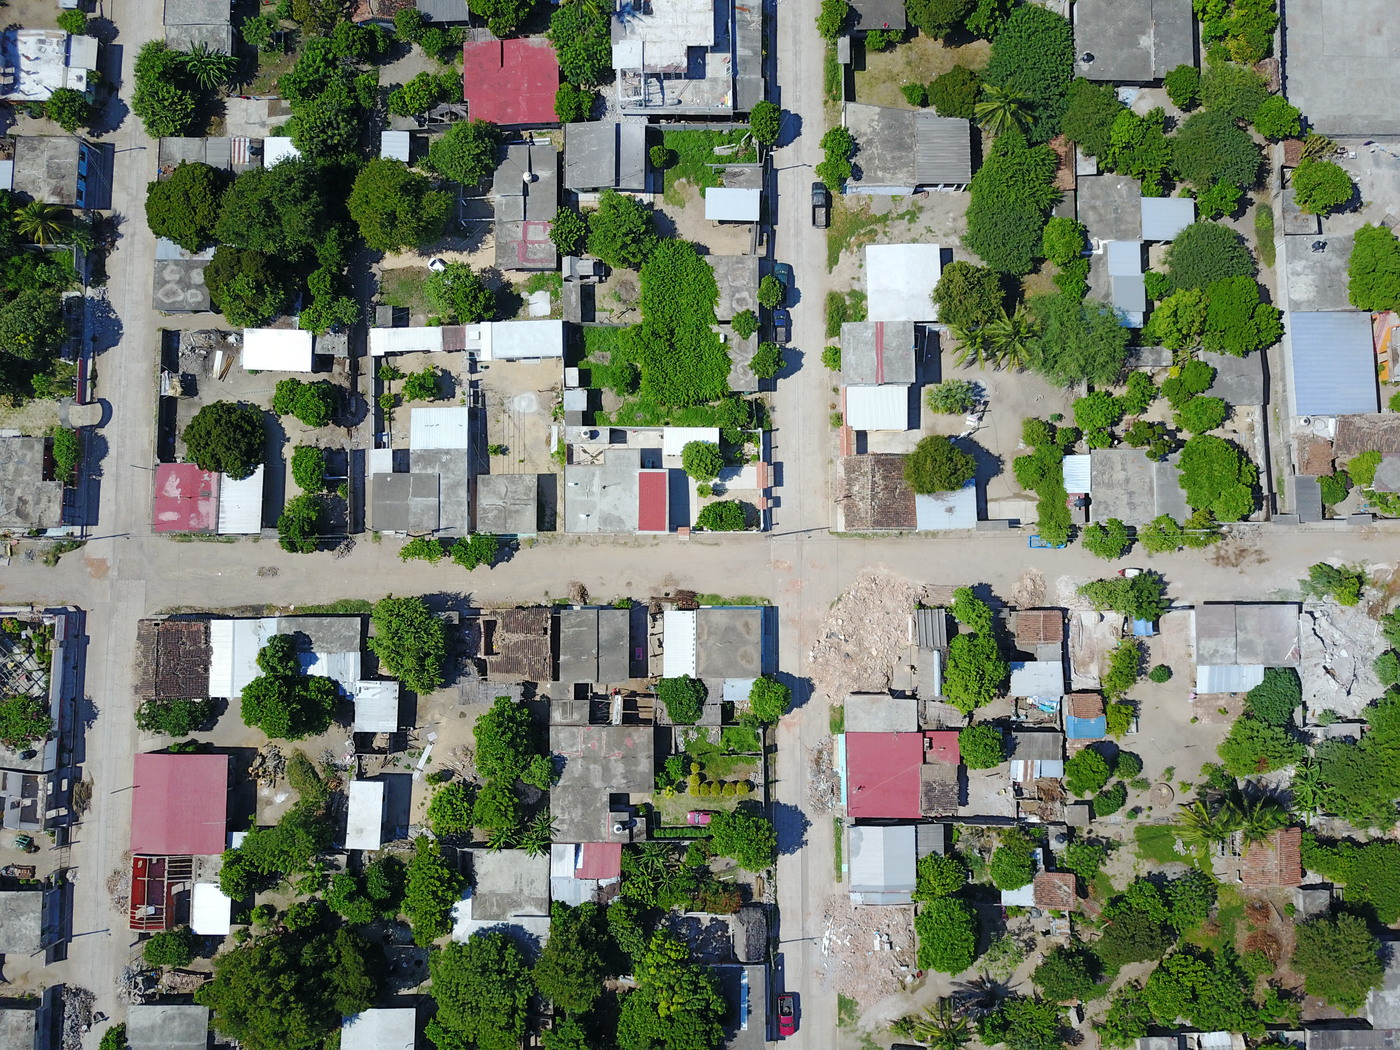
\includegraphics[width=\textwidth]{images/santamaria-sample.jpg}
    \end{subfigure}
  \caption{Santa Mar\'ia Xadani.}
  \label{fig:santamaria}
\end{figure}

\begin{figure}[!h]
  \centering
    \begin{subfigure}{.8\textwidth}
        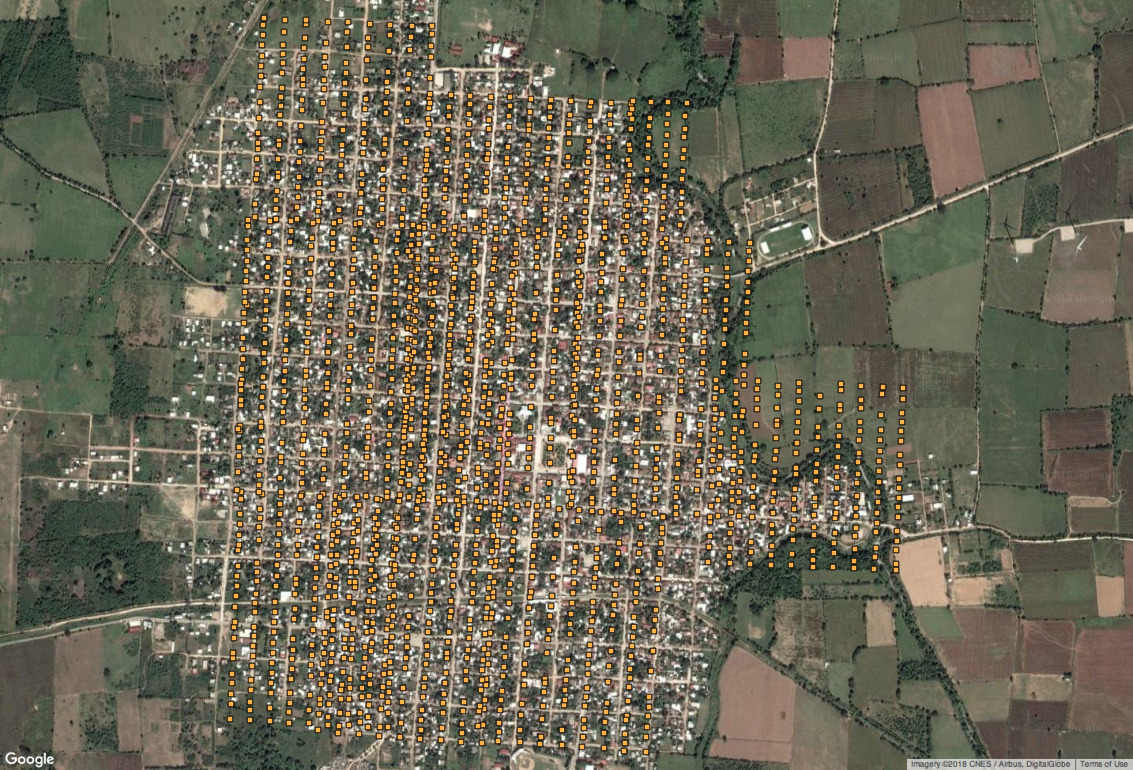
\includegraphics[width=\textwidth]{images/union-satellite.jpg}
    \end{subfigure}
    \begin{subfigure}{.8\textwidth}
        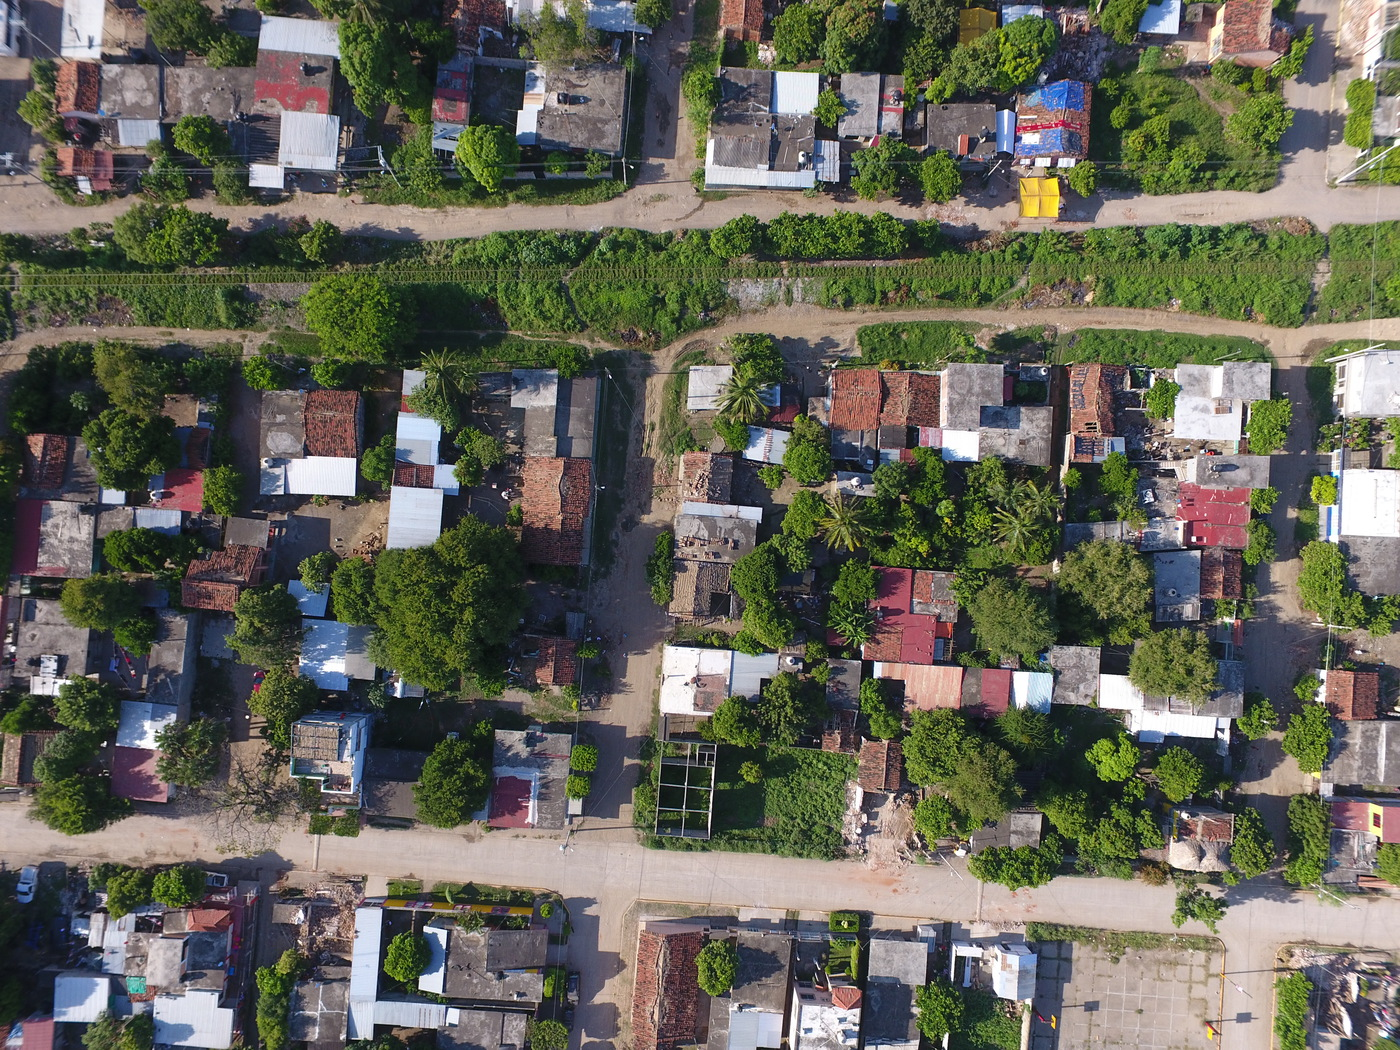
\includegraphics[width=\textwidth]{images/union-sample.jpg}
    \end{subfigure}
  \caption{Uni\'on Hidalgo.}
  \label{fig:union}
\end{figure}

As we can see from Figures \ref{fig:juchitan}, \ref{fig:santamaria}, and \ref{fig:union}, drones flew in regular patterns forming a lattice of points, these clouds of information distribute evenly around the towns of interest. Given this distribution, it was reasonable to hypothesize that there was an underlying similarity between images of the same town. This similarity might be caused by the light conditions during the exposure that tend to have less variance among similar times and places. A limitation found was that the size of the images\footnote{Raw images are $4000\times3000$ pixels, and three color channels each.} prevented us from computing regular metrics such as the Euclidian distance between a pair of images. To overcome this problem, the information from the pixels of each image was flattened into a vector comprising the means and standard deviations for each color channel. In summary, for each image, we obtained a vector of six components.\\

To test our hypothesis over this new set of data, we used an algorithm known as t-Distributed Stochastic Neighbor Embedding (t-SNE), introduced by Laurens van der Maaten \cite{t-sne}. This technique allowed us to visualize the information in a two-dimensional plane\footnote{The interest of being able to represent the images in a two-dimensional structure comes from the idea of simplifying things for better understanding. High dimensional data usually lies in hidden low dimensional manifolds, techniques like t-SNE give us insights about this underlying structure.}. As we expected the images of the different towns cluster in this low dimensional representation. We show our results in Figure \ref{fig:tsne}.\\

The outcome of this experiment gave us a reason to model our methodology around the characteristics of the data. Using the information of a certain town and later testing the model with data from another one allowed us to evaluate the generalization capacity of the model.\\


\begin{figure}[!h]
  \centering
  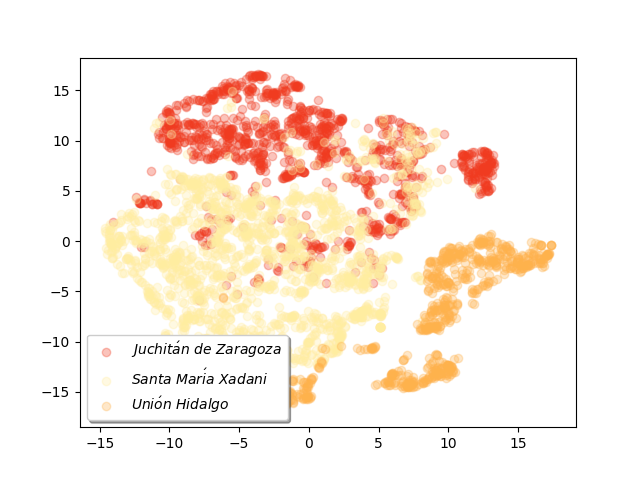
\includegraphics[width=1\textwidth]{images/t-sne-bis.png}
  \caption{T-sne diagram.}
  \label{fig:tsne}
\end{figure}

\section{Experiment}

We needed a benchmark to test the effectiveness of our method. To this end, we used classic computer vision methods on our dataset. We extracted simple features from the images, and then we trained a classification model on the resulting data\footnote{Spending more time on feature engineering on the pictures would undoubtedly lead to better results. However, it was not the scope of the present work.}. The final purpose was to show how the methods compare out of the box with little extra effort.\\

We considered three types of features. First, we used a method known as Histogram of Oriented Gradients (HOG), introduced by William T. Freeman and Michal Roth \cite{MERL_TR94-03}. It consists of studying the slopes of the intensity of the pixels in a dense grid of the image. The feature space that this method output depends on the size of the lattice. Then, to test more straightforward features, we extracted the means and the standard deviations from each of the color channels in the same fashion that we did with t-SNE in the exploratory analysis. We additionally decided to consider the color channel means alone as a different feature set. Finally, we trained a random forest for each of these three sets of attributes.\\

\begin{figure}[!h]
  \centering
    \begin{subfigure}{.24\textwidth}
        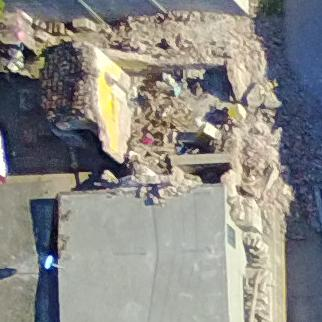
\includegraphics[width=\textwidth]{images/damaged1.jpg}
    \end{subfigure}
    \begin{subfigure}{.24\textwidth}
        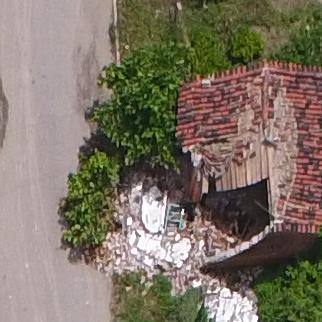
\includegraphics[width=\textwidth]{images/damaged2.jpg}
    \end{subfigure}
    \begin{subfigure}{.24\textwidth}
        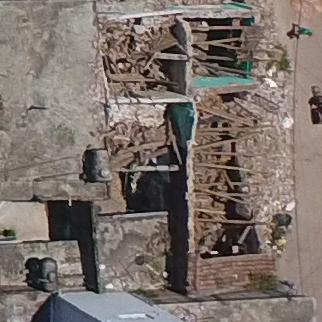
\includegraphics[width=\textwidth]{images/damaged3.jpg}
    \end{subfigure}
    \begin{subfigure}{.24\textwidth}
        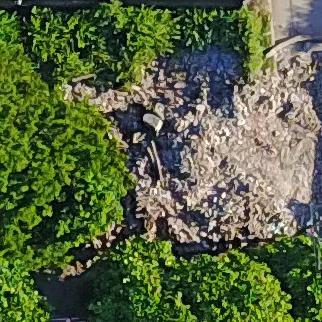
\includegraphics[width=\textwidth]{images/damaged4.jpg}
    \end{subfigure}
    %
    \begin{subfigure}{.24\textwidth}
        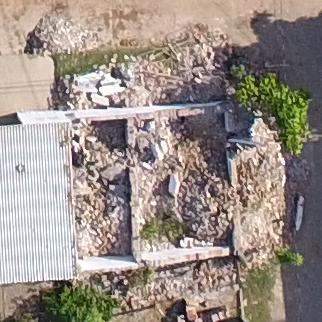
\includegraphics[width=\textwidth]{images/damaged5.jpg}
    \end{subfigure}
    \begin{subfigure}{.24\textwidth}
        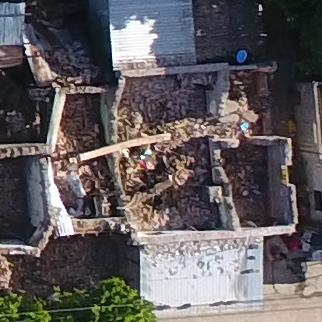
\includegraphics[width=\textwidth]{images/damaged6.jpg}
    \end{subfigure}
    \begin{subfigure}{.24\textwidth}
        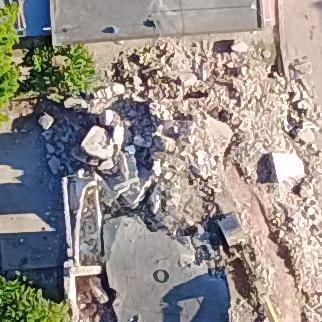
\includegraphics[width=\textwidth]{images/damaged7.jpg}
    \end{subfigure}
    \begin{subfigure}{.24\textwidth}
        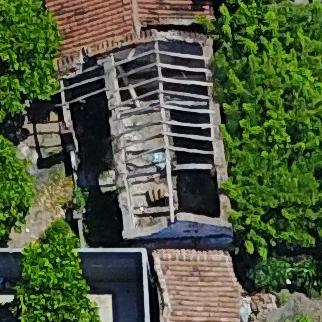
\includegraphics[width=\textwidth]{images/damaged8.jpg}
    \end{subfigure}
  \caption{Sample images from the damaged training set.}
  \label{fig:damaged}
\end{figure}


We reduced the problem to binary classification by selecting only two labels; a \textit{damage} tag when the samples showed clear infrastructure damage, and a \textit{no damage} tag when we saw no visible damage. We show some examples for both categories in Figures \ref{fig:damaged} and \ref{fig:nondamaged}. We used the application detailed in the previous chapter to crop and classify 200 square patches from the images in each of the towns. To keep the classes balanced, we chose 100 images for each class. Every sample was $327\times327$ pixels, and we assigned a tag manually for each of them. After the tagging process, we had 600 labeled images that we will refer to as \textit{our dataset} through the rest of this chapter. The information was stored in the relational database and reviewed for data consistency.\\

\begin{figure}[!h]
  \centering
    \begin{subfigure}{.24\textwidth}
        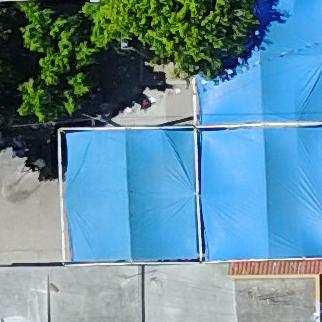
\includegraphics[width=\textwidth]{images/nondamaged1.jpg}
    \end{subfigure}
    \begin{subfigure}{.24\textwidth}
        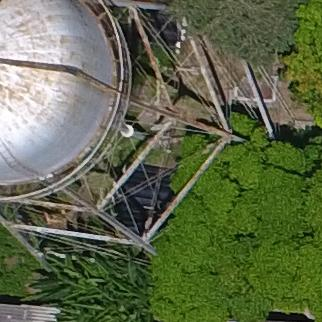
\includegraphics[width=\textwidth]{images/nondamaged2.jpg}
    \end{subfigure}
    \begin{subfigure}{.24\textwidth}
        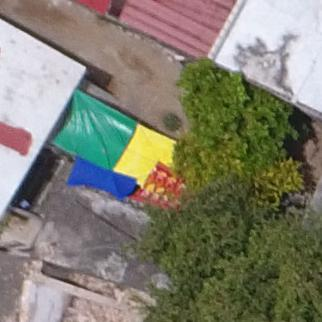
\includegraphics[width=\textwidth]{images/nondamaged3.jpg}
    \end{subfigure}
    \begin{subfigure}{.24\textwidth}
        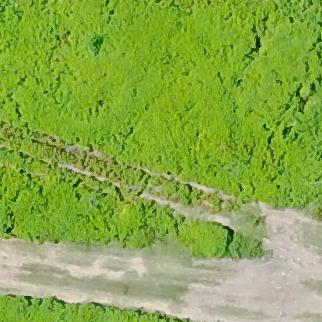
\includegraphics[width=\textwidth]{images/nondamaged4.jpg}
    \end{subfigure}
    %
    \begin{subfigure}{.24\textwidth}
        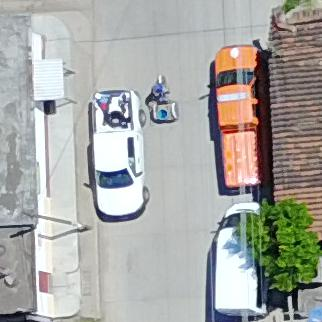
\includegraphics[width=\textwidth]{images/nondamaged5.jpg}
    \end{subfigure}
    \begin{subfigure}{.24\textwidth}
        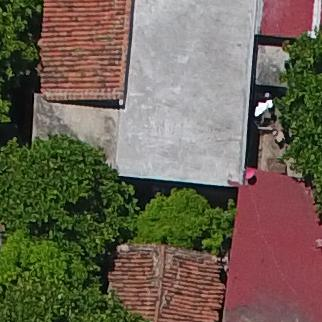
\includegraphics[width=\textwidth]{images/nondamaged6.jpg}
    \end{subfigure}
    \begin{subfigure}{.24\textwidth}
        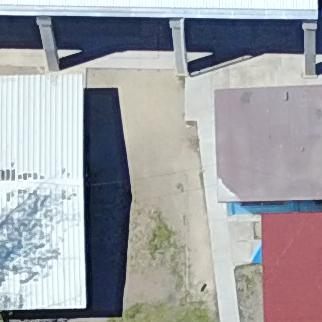
\includegraphics[width=\textwidth]{images/nondamaged7.jpg}
    \end{subfigure}
    \begin{subfigure}{.24\textwidth}
        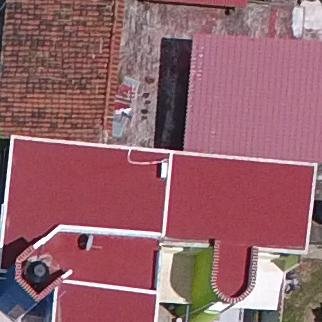
\includegraphics[width=\textwidth]{images/nondamaged8.jpg}
    \end{subfigure}
  \caption{Sample images from the non damaged training set.}
  \label{fig:nondamaged}
\end{figure}

As mentioned earlier, we studied three different towns, so we assembled different datasets using a different permutation each time. In the case of the classic computer vision methods, we used two towns to train the model and the remaining one to test the trained model. In the case of the transfer learning model, we used the images of one town to retrain the model, the images of another town to validate the model during the training stage, and the remaining town to test the trained model. In all cases, we tested every single image in the testing town against the model.\\

One of the difficulties that we found during our research process was that several images might depict the same collapsed building (Figure \ref{fig:compare}). This event could happen when the drone flew over the same territory in different routes. During the tagging stage, we inspected the images for damaged areas, however, despite our efforts, it was impossible to obtain a set of pictures in which every single one was completely independent of the rest. This fact shaped our validation process.\\

\begin{figure}[!ht]
  \centering
  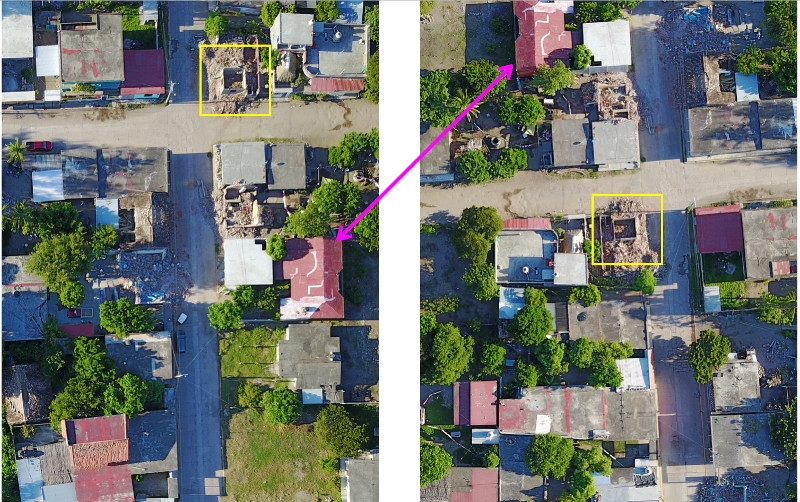
\includegraphics[width=1\textwidth]{images/compare.jpg}
  \caption{An example of the same building in two diferent images. The drone flew over the same place in different moments and directions.}
  \label{fig:compare}
\end{figure}

A classical approach would be to divide the dataset into two parts; training and testing sets, the model is trained with the former, and then tested against the latter. This method is not used in practice because data is usually scarce and we would like to take the most of it. A better option is n-fold crossed-validation in which we repeat a similar approach n times and average the outcomes. This process makes more likely to train the model with every data point and average out errors that may appear by chance. However, n-fold crossed-validation does not suit our case because of the nature of our dataset. As a consequence of the patterns in which the drones overfly the area, some buildings appear several times in the dataset even though the original pictures were not the same. If we apply a technique such as cross-validation, it would be very likely to have the same building both in training and in the testing sets. This situation would lead to having very high accuracies for our model but not such good performance in a real setting.\\

Another thing to be considered is that while traditional supervised classification methods need to divide the dataset into two parts to perform the validation, machine learning methods often require three sets instead, namely train, validation, and test. The validation set is used during the training stage to fine tune the hyperparameters of the model, and then the testing set is used to see how our model deals with previously unseen data. We manage to elegantly avoid the problem of having repeated data on each of the datasets by using the fact of having information from three completely independent settings. We trained models feeding them with different training set sizes and testing them against a set of a fixed size. In summary, we trained a model for each combination of a method, a training set size, and town permutation.\\

\subsection{Classic Computer Vision}

We extracted the HOG features using an implementation from the Python package scikit-image \cite{scikit-learn}. We used eight orientations, and a $16\times16$ pixel window. Each town was selected once for testing, in table \ref{table:classic}, we show the codes that we use in Figure \ref{fig:classic} to show the results that we obtained.\\

\begin{table}
  \caption{Permutation codes.}
  \resizebox{\textwidth}{!}{%
  \begin{tabular}{|c|c|c|}
    \hline
    Train Set                                      &Test Set               &Code \\ \hline
    Juchit\'an de Zaragoza, Uni\'on Hidalgo        &Santa Mar\'ia Xadani   &JU-S \\ \hline
    Juchit\'an de Zaragoza, Santa Mar\'ia Xadani   &Uni\'on Hidalgo        &JS-U \\ \hline
    Santa Mar\'ia Xadani, Uni\'on Hidalgo          &Juchit\'an de Zaragoza &SU-J \\ 
    \hline
  \end{tabular}}
  \label{table:classic}
\end{table}

\begin{figure}[ht]
  \centering
    \begin{subfigure}{.49\textwidth}
        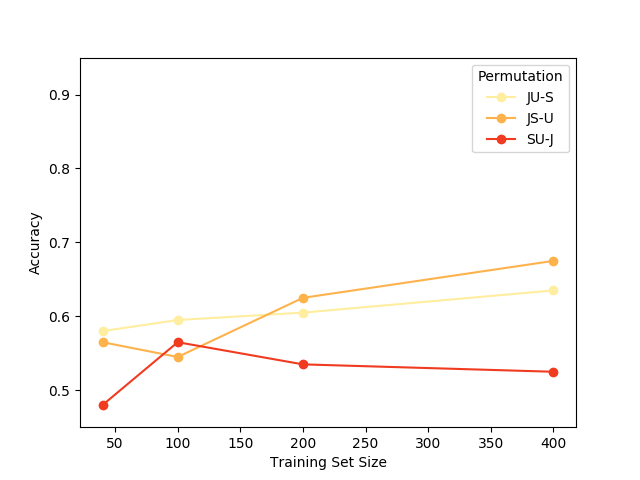
\includegraphics[width=\textwidth]{images/classic-hog.png}
        \caption{Histogram of Oriented Gradients}
    \end{subfigure}
    \begin{subfigure}{.49\textwidth}
        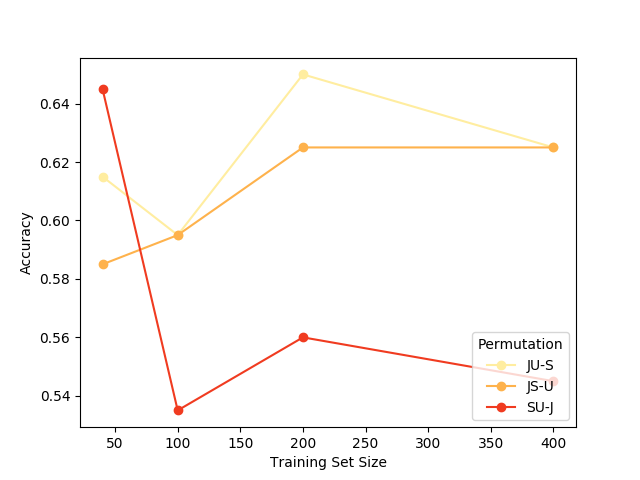
\includegraphics[width=\textwidth]{images/classic-means.png}
        \caption{Means}
    \end{subfigure}
    %
    \begin{subfigure}{.49\textwidth}
        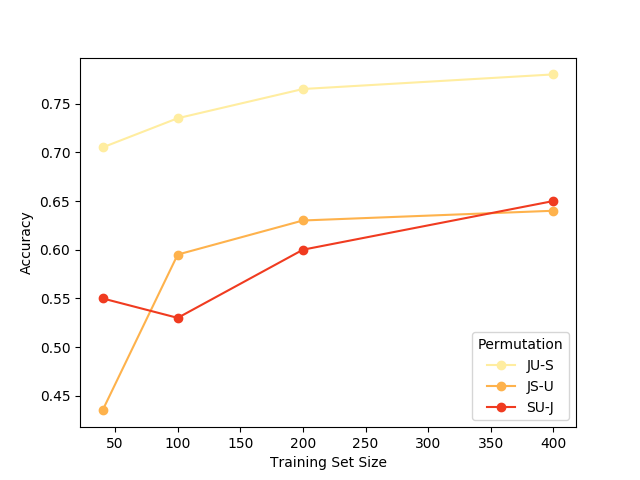
\includegraphics[width=\textwidth]{images/classic-meanstd.png}
        \caption{Means + Standard Deviation}
    \end{subfigure}
  
  \caption{Training example using classic computer vision models.}
  \label{fig:classic}
\end{figure}

It was surprising that the model that showed the best performance was the one in which we considered means and standard deviations. We expected that the specialized features of the HOG model to perform better than a simple mean and standard deviation extraction. We think that the reason behind this was that the HOG features were designed to find objects in images, but they are not well suited for aerial images and the textures that characterize debris. As we expected, increasing the size of the training set results in improving the performance of the trained model. In particular, we noticed that the worse performing models were the ones using Juchit\'an de Zaragoza as the training set, a hypothesis is that the pictures from Santa Mar\'ia Xadani and Uni\'on Hidalgo do not generalize so well. The best performing model achieved 78\% accuracy and used Santa Mar\'ia Xadani as the testing set and all of the remaining 400 images to train. The worse performing model achieved 43.5\% and used Uni\'on Hidalgo to test with only 40 images in the training set which is particularly unfortunate considering we are dealing with binary classifiers.\\

\subsection{Transfer Learning}

In the case of transfer learning, we have three types of sets and three towns. This fact makes six different possible configurations. Thus six different models for each training set size. We retrained the Inception model using our dataset and 1000 training steps\footnote{We empirically noticed that further increase in the number of training steps did not improve the final accuracy of the model.}.\\

\begin{table}[h!]
  \caption{Permutation codes.}
  \resizebox{\textwidth}{!}{%
  \begin{tabular}{|c|c|c|c|}
    \hline
    Train Set              &Validate Set           &Test Set               &Code  \\ \hline
    Uni\'on Hidalgo        &Juchit\'an de Zaragoza &Santa Mar\'ia Xadani   &U-J-S \\ \hline
    Uni\'on Hidalgo        &Santa Mar\'ia Xadani   &Juchit\'an de Zaragoza &U-S-J \\ \hline
    Juchit\'an de Zaragoza &Uni\'on Hidalgo        &Santa Mar\'ia Xadani   &J-U-S \\ \hline
    Juchit\'an de Zaragoza &Santa Mar\'ia Xadani   &Uni\'on Hidalgo        &J-S-U \\ \hline
    Santa Mar\'ia Xadani   &Uni\'on Hidalgo        &Juchit\'an de Zaragoza &S-U-J \\ \hline
    Santa Mar\'ia Xadani   &Juchit\'an de Zaragoza &Uni\'on Hidalgo        &S-J-U \\
    \hline
  \end{tabular}}
\end{table}

\begin{figure}[h]
  \centering
  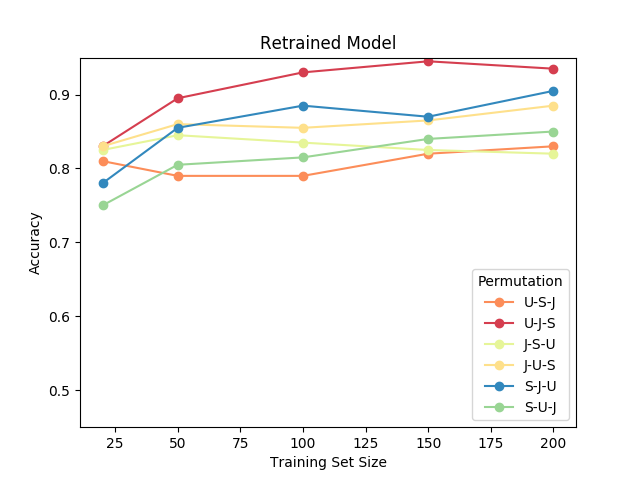
\includegraphics[width=1\textwidth]{images/validation-plot.png}
  \label{fig:validaton-plot}
  \caption{Results of our experiment. As we expected, the graph shows a positive correlation between the accuracy and the number of training samples.}
\end{figure}

\subsection{Threshold Selection}

A binary classifier assigns a real number in the interval $[0,1]$. To decide which tag to assign to each prediction we must choose a decision threshold. A tool that is often used to select such threshold is a Receiver Operating Characteristic curve (ROC curve). It was first proposed during World War II to measure the ability of a receiver operator to detect an enemy ship, where it took its name \cite{GreenSwets66}.

When dealing with a binary classifier, we want to predict a condition $p$. If the outcome of our classification is $p$ and the real value is also $p$ we call that a true positive (TP), if the actual value is instead $n$, we call that a false positive. Conversely, we assign names for a true negative (TN) and a false negative when we predict $n$ as the outcome for our classifier. We call true positive rate (TPR) or \textit{sensitivity} to the ratio between the outcomes correctly predicted as $p$ and the number of elements that are indeed $p$. We are also interested in the false positive rate (FPR) or \textit{specificity}, which is the proportion of incorrectly assigning $p$ given that the condition is $n$. In a ROC curve, we plot the sensitivity as a function of the specificity; it is used to select a decision threshold and have a tradeoff between detecting as many positives and having as little false alarms as possible. There is an additional feature of interest, the area under the ROC curve (AUC) is often used for model comparison, the closer the value is to $1$ the better.\\

There is no correct way to select a decision threshold. It depends on the application at hand. For instance, when we are dealing with disease diagnosis, a screening test should be very sensitive whereas a confirmatory test should be very specific. In our case we want our classifier to be very sensitive because there is not as much overhead to have false alarms. In Figure \ref{fig:roc} we show the ROC curves for each of the transfer learning models. To build them, the prediction for each test image was recorded for each permutation among the different training set sizes. Therefore, we have a ROC curve for every training set size. As we can see, the area under the curve is very close to $1$ in every case, and it increases as the training set size increases.\\

\begin{figure}[!h]
  \centering
    \begin{subfigure}{.48\textwidth}
        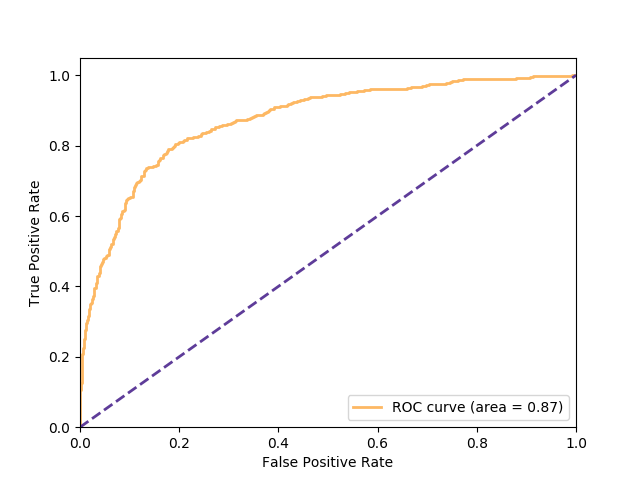
\includegraphics[width=\textwidth]{images/score-10-roc.png}
        \caption{Training Set Size: 20 Images}
    \end{subfigure}
    %
    \begin{subfigure}{.48\textwidth}
        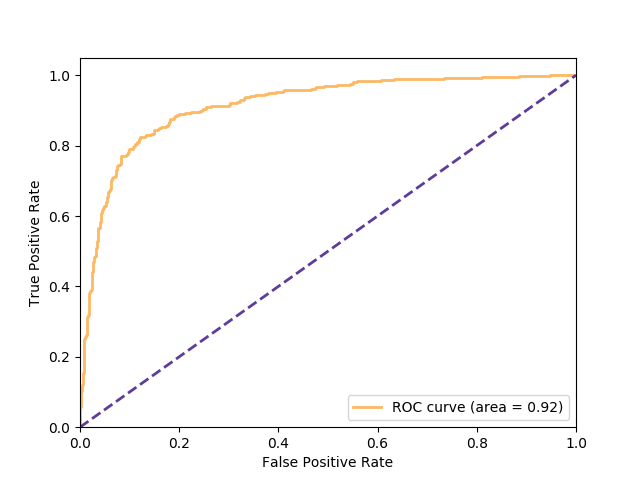
\includegraphics[width=\textwidth]{images/score-25-roc.png}
        \caption{Training Set Size: 50 Images}
    \end{subfigure}
    %
    \begin{subfigure}{.48\textwidth}
        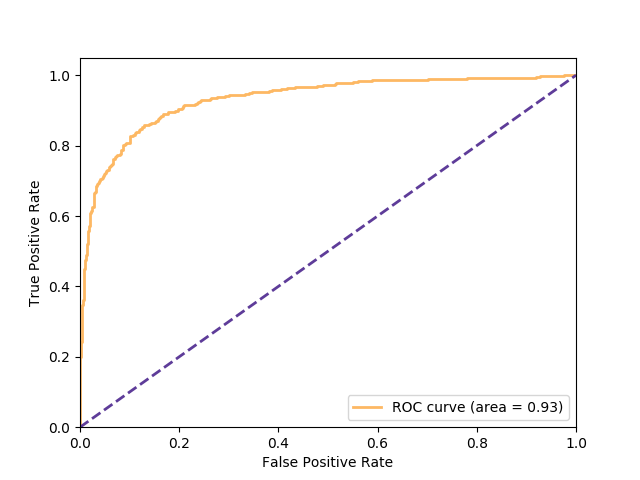
\includegraphics[width=\textwidth]{images/score-50-roc.png}
        \caption{Training Set Size: 100 Images}
    \end{subfigure}
    %
    \begin{subfigure}{.48\textwidth}
        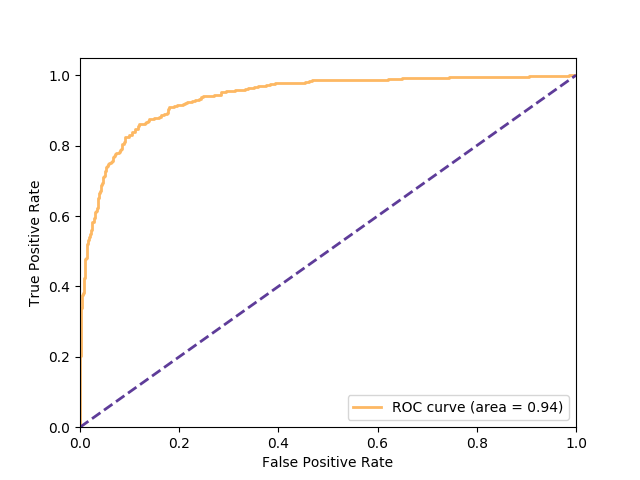
\includegraphics[width=\textwidth]{images/score-75-roc.png}
        \caption{Training Set Size: 150 Images}
    \end{subfigure}
    %
    \begin{subfigure}{.48\textwidth}
        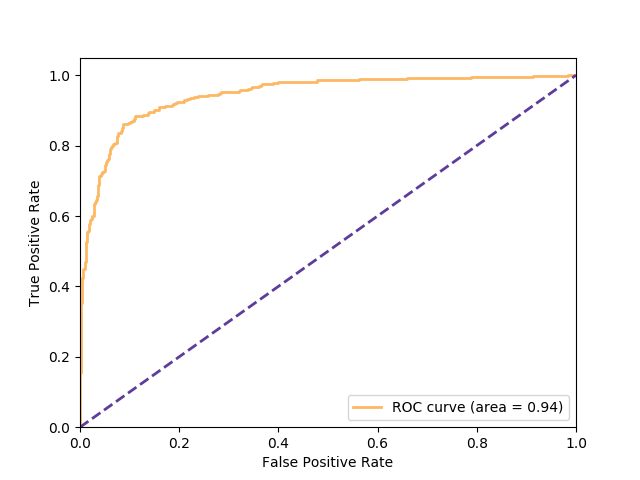
\includegraphics[width=\textwidth]{images/score-100-roc.png}
        \caption{Training Set Size: 200 Images}
    \end{subfigure}
  
  \caption{Receiver operating characteristic curves for the different training set sizes. We show the performance of the transfer learning models using Inception as the base.}
  \label{fig:roc}
\end{figure}







